\PassOptionsToPackage{type=CC,modifier=by,version=4.0}{doclicense}
\documentclass[conference,a4paper,flushend]{cs-techrep}
\pdfoutput=1 % pdflatex hint for arxiv.org (within first 5 lines)

% Class cs-techrep.cls loads biblatex / biber with predefined options
\addbibresource{embedded.bib}       % its content is declared below, embedded within this tex-file
\addbibresource{webdev_commons.bib} % includes REST, React, Angular, Vue, Svelte, Docker, AWS-*, Socket.IO, and many more!
\addbibresource{cpn_all_all.bib}    % includes all previous CyberLytics@OTH-AW technical reports

% ======================================================================
% EDIT THESE:

\cstechrepAuthorListTex{Andreas Fillenberg, Franziska Rubenbauer, Martin Zizler,\\ Christian Süß, Lukas Rupp, Christoph P.\ Neumann\,\orcidlink{0000-0002-5936-631X}}
\cstechrepAuthorListBib{Andreas Fillenberg, Franziska Rubenbauer, Martin Zizler, Christian Süß,\\ Lukas Rupp, Christoph P.\ Neumann}

% Capitalization: https://capitalizemytitle.com/style/Chicago/
\cstechrepTitleTex{MuskMonitor: Eine MFRN-basierte Webanwendung zur Vorhersage der Tesla Stock Daten}
 % IF you need manual linebreaks in the titel, then clone the title without linebreaks for BibTeX:
\cstechrepTitleBib{{\cstechrepTitleTex}}

\cstechrepDepartment{CyberLytics\-/Lab at the Department of Electrical Engineering, Media, and Computer Science}
%\cstechrepDepartment{CyberLytics\-/Lab an der Fakultät Elektrotechnik, Medien und Informatik} % DE
\cstechrepInstitution{Ostbayerische Technische Hochschule Amberg\-/Weiden}
\cstechrepAddress{Amberg, Germany}
%\cstechrepAddress{Amberg, Deutschland} % DE
\cstechrepType{Technical Report}
%\cstechrepType{Technischer Bericht} % DE
\cstechrepYear{2024}
\cstechrepMonth{12}
\cstechrepNumber{CL-TR-\cstechrepYear{}-42}
\cstechrepLang{ngerman}  % en-US
%\cstechrepLang{ngerman} % DE

% Special remark on babel/csquotes terminology in regard with US-vs-UK:
% en-US  = [english]/[american]/[usenglish] (+ [canadian])
% en-UK  =           [british] /[ukenglish] (+ [australian]) <OXFORD>
% For cs-techrep (like ACM), the recommended english variant is en-US!

% DO NOT DELETE THIS:
\filecontentsForceExpansion|[] % force command expansion inside a filecontents* environment
\begin{filecontents*}[overwrite]{selfref.bib}
    @TECHREPORT{selfref,
        author = {|cstechrepAuthorListBib},
        title  = {\cstechrepTitleBib},
        institution = {\cstechrepInstitution, \cstechrepDepartment},
        type   = {\cstechrepType},
        number = {\cstechrepNumber},
        year   = {|cstechrepYear},
        month  = {|cstechrepMonth},
        langid  = {|cstechrepLang},
    }
\end{filecontents*}

% ======================================================================
% EDIT THIS:

\begin{filecontents}[overwrite]{embedded.bib}
@misc{noauthor_cardiffnlptwitter-roberta-base-sentiment-latest_2024,
    title = {cardiffnlp/twitter-roberta-base-sentiment-latest · {Hugging} {Face}},
    url = {https://huggingface.co/cardiffnlp/twitter-roberta-base-sentiment-latest},
    abstract = {We’re on a journey to advance and democratize artificial intelligence through open source and open science.},
    urldate = {2024-12-03},
    month = jan,
    year = {2024},
}
@misc{loureiro_timelms_2022,
    title = {{TimeLMs}: {Diachronic} {Language} {Models} from {Twitter}},
    shorttitle = {{TimeLMs}},
    url = {http://arxiv.org/abs/2202.03829},
    doi = {10.48550/arXiv.2202.03829},
    abstract = {Despite its importance, the time variable has been largely neglected in the NLP and language model literature. In this paper, we present TimeLMs, a set of language models specialized on diachronic Twitter data. We show that a continual learning strategy contributes to enhancing Twitter-based language models’ capacity to deal with future and out-of-distribution tweets, while making them competitive with standardized and more monolithic benchmarks. We also perform a number of qualitative analyses showing how they cope with trends and peaks in activity involving specific named entities or concept drift. TimeLMs is available at https://github/. com/cardiffnlp/timelms.},
    language = {en},
    urldate = {2024-12-03},
    publisher = {arXiv},
    author = {Loureiro, Daniel and Barbieri, Francesco and Neves, Leonardo and Anke, Luis Espinosa and Camacho-Collados, Jose},
    month = apr,
    year = {2022},
    note = {arXiv:2202.03829 [cs]},
    keywords = {Computer Science - Artificial Intelligence, Computer Science - Computation and Language},
}

\end{filecontents}

\usepackage{fontawesome} % i.a., \faWarning{}
\usepackage{relsize}     % i.a., \textsmaller{...}
\usepackage{lipsum}      % for blindtext

% ======================================================================

% cf. https://ctan.org/pkg/acronym
% Usage:
% singular, within sentence       = \ac{gui}
% singular, beginning of sentence = \Ac{gui}
% plural, within sentence         = \acp{gui}
% plural, beginning of sentence   = \Acp{gui}

% https://www.silbentrennung24.de/
% https://www.hyphenation24.com/

\begin{document}
\selectlanguage{\cstechrepLang}

\maketitle

\begin{abstract}
MuskMonitor ist eine Webanwendung, die zeigt, wie Elon Musks Tweets den Tesla-Aktienkurs beeinflussen. Die zentrale Logik der Anwendung kombiniert Sentiment-Analysen von Tweets mit historischen Kursverläufen der Aktie, um Prognosen für die Zukunft zu erstellen. Die Zielgruppe der Anwendung sind Trader und Analysten, die datenbasierte Entscheidungen treffen oder tiefere Marktanalysen durchführen möchten. Die Architektur umfasst einen Flask-Server im Backend, geschrieben in Python, sowie ein React-Frontend. Die Daten werden in einer MongoDB gespeichert.
\end{abstract}

% A list of IEEE Computer Society appoved keywords can be obtained at
% http://www.computer.org/mc/keywords/keywords.htm
\begin{IEEEkeywords}
Webanwendung – Aktienmarkt – X – React – Python – MongoDB
\end{IEEEkeywords}

\section{Einführung und Ziele}

Der Einfluss von Social-Media-Posts auf die Finanzmärkte, insbesondere von Persönlichkeiten wie Elon Musk, ist ein bekanntes, aber schwer messbares Phänomen. Die Herausforderung besteht darin, diese Effekte auf eine verständliche und datenbasierte Weise darzustellen. Das Hauptziel von MuskMonitor ist es, eine potenzielle Korrelation zwischen bedeutenden Tweets und den anschließenden Aktienkursveränderungen sichtbar zu machen. Viele bestehende Methoden sind manuell oder liefern unklare Ergebnisse, was sie für Investoren nur bedingt nützlich macht.

\textbf{Mission Statement: }
MuskMonitor ist eine Webanwendung, die es Anlegern und Analysten ermöglicht, den Einfluss von Elon Musks Tweets auf den Tesla-Aktienkurs zu analysieren und vorherzusagen. Wir schaffen eine intuitive, datengetriebene Plattform, die historische Kursdaten mit Sentiment-Analysen kombiniert und so Mehrwert für datenbasierte Entscheidungen bietet.

\textbf{Kontextabgrenzung: }  
Die Anwendung konzentriert sich ausschließlich auf Elon Musks Tweets und deren Zusammenhang mit dem Tesla-Aktienkurs. Diese klar definierte und technisch umsetzbare Grundlage dient als Ausgangspunkt. Eine Erweiterung auf andere prominente Persönlichkeiten ist perspektivisch denkbar, bleibt jedoch außerhalb des aktuellen Projektumfangs.




\section{State-of-the-art}
\subsection{Sentiment-Analyse}
Die Sentiment-Analyse wird mithilfe des Huggingface-Modells Twitter-RoBERTa-base durchgeführt \cite{noauthor_cardiffnlptwitter-roberta-base-sentiment-latest_2024}. Das Modell basiert auf dem RoBERTa-Modell, das mit über ~124 Millionen Tweets trainiert wurde, die zwischen Januar 2018 und Dezember 2021 veröffentlicht wurden, und anschließend auf dem Sentiment-Analyse-Teil des TweetEval-Benchmarks finegetuned wurde. Die RoBERTa-Architektur basiert auf der Arbeit von Loureiro et al. \cite{loureiro_timelms_2022}, welche TimeLMs als neue Modellart einführt. TimeLMs wurden als Modelle entwickelt, die kontinuierlich alle 3 Monate mit neuen Twitter-Daten weitertrainiert werden. Dieses Training lief bis Ende 2021, wodurch TimeLMs zeitliche Entwicklungen der Sprache adressieren und sich besser an neue Trends und Bedeutungsverschiebungen anpassen. Daher eignen sie sich besonders gut für die Stimmungsanalyse auf Twitter.

Das RoBERTa Modell verwendet des weiteren Masked Language Modeling (MLM). MLM ist eine Technik, bei der während des Trainings zufällig ausgewählte Tokens im Text durch einen Platzhalter wie <mask> ersetzt werden. Das Modell wird darauf trainiert, die maskierten Tokens anhand des umgebenden Kontexts korrekt vorherzusagen. Dieses Verfahren wurde ursprünglich in der BERT-Architektur eingeführt und in der RoBERTa-Architektur weiter optimiert, auf der die TimeLMs basieren.

Statisch vortrainierte Modelle wie BERT oder RoBERTa verlieren im Vergleich zu TimeLMs an Relevanz, wenn sich die Sprache schnell verändert – etwa während der COVID-19-Pandemie. TimeLMs hingegen bleiben durch kontinuierliches Training aktuell und passen sich zeitlichen Sprachveränderungen an. Ein alternatives Twitter-basiertes Modell ist BERTweet, das jedoch nur mit Tweets bis 2019 trainiert wurde und keine diachrone Komponente besitzt. Aus diesem Grund ist BERTweet bei zeitabhängigen Aufgaben und auf aktuellen Daten den TimeLMs unterlegen.

Zudem unterscheiden sich TimeLMs von domänenunabhängigen Modellen wie GPT-2 oder GPT-3, die nicht speziell für soziale Medien entwickelt wurden. Aufgrund ihres allgemeinen Trainings erfassen diese Modelle den informellen und dynamischen Sprachstil von Tweets weniger präzise.

\subsection{Aktienkursvorhersage}
Die Vorhersage von Aktienkursen erfolgt mithilfe eines Long-Short-Term-Memory-Modells (LSTM), das auf historischen Daten basiert, die täglich zu den offenen, hohen, niedrigen und Schlusskursen der Tesla-Aktien sowie dem Handelsvolumen aus einer MongoDB-Datenbank gesammelt wurden. Diese Daten werden zunächst normalisiert, um sie auf eine einheitliche Skala zu bringen, was die Stabilität und Genauigkeit des Modells verbessert. Anschließend werden die Daten aufgeteilt: 75 \% werden für das Training genutzt und 25 \% für die Validierung.

Das LSTM-Modell wird mit den Kursdaten der letzten 60 Tage trainiert, um die Kursentwicklung für den nächsten Tag vorherzusagen. LSTM-Netzwerke eignen sich besonders für die Modellierung von Zeitreihendaten, da sie in der Lage sind, langfristige Abhängigkeiten zu erkennen – eine wesentliche Eigenschaft von Aktienkursen, die oft auf früheren Mustern und Trends basieren. Während des Trainings minimiert das Modell den Fehler zwischen den Vorhersagen und den tatsächlichen Werten mithilfe der Verlustfunktion Mean Squared Error (MSE).

Nach Abschluss des Trainings wird das Modell auf Testdaten evaluiert, wobei die Leistung anhand des Root Mean Squared Error (RMSE) gemessen wird. Ein niedriger RMSE-Wert zeigt, dass das Modell die tatsächliche Kursentwicklung präzise vorhersagen kann. Schließlich werden die Vorhersagen grafisch mit den realen Kursen verglichen, um die Leistung des Modells visuell darzustellen. Diese Methode verdeutlicht, wie LSTM-Netzwerke komplexe, nicht-lineare Muster der Finanzmärkte erkennen und auf dieser Basis zuverlässige Vorhersagen für die zukünftige Kursentwicklung treffen können.

\section{Architekturziele} % \textbar{} \textquote{Architekturziele}}
\textbf{Prognose-Genauigkeit:}  Das Prognosemodell zielt darauf ab, möglichst präzise Vorhersagen zu Aktienkursveränderungen zu liefern. Diese basieren auf einer Kombination aus historischen Kursdaten.
\textbf{Visualisierung:} Für eine benutzerfreundliche Darstellung werden die Daten klar visualisiert. Dies umfasst sowohl historische Kursverläufe als auch die Auswirkungen einzelner Tweets, um Zusammenhänge schnell und intuitiv erfassbar zu machen.
\textbf{Skalierbarkeit und Robustheit:} Die Anwendung wird in der Cloud bereitgestellt, um eine zuverlässige Nutzung auch bei steigender Benutzeranzahl und wachsendem Datenvolumen zu gewährleisten.
\textbf{Datenqualität:} Um eine konsistente und verlässliche Analyse zu ermöglichen, werden Tweets und Kursdaten regelmäßig abgerufen, bereinigt und aufbereitet.
\textbf{Datenakquise:} Aufgrund eines begrenzten Zugriffs auf die Twitter API wurden alternative Datenquellen genutzt, wie beispielsweise historische Datensätze aus Open-Source-Plattformen.
\textbf{Sentiment-Analyse:} Die Stimmungsbewertung von Tweets basiert auf einem robusten Modell, das spezifische Sprachmuster und Kontextfaktoren berücksichtigt, um eine präzise Sentiment-Einschätzung zu gewährleisten.
\textbf{Datenintegration:} Eine präzise und performante Integration der Tweets und Kursdaten erfolgt über Zeitstempel, um eine zuverlässige Verbindung zwischen den Datenquellen herzustellen.

Durch diese Herangehensweise wird die Grundlage für ein Minimum Viable Product (MVP) geschaffen. Dieses MVP stellt wesentliche Funktionen wie Kursprognosen, Sentiment-Analysen und die Visualisierung historischer Entwicklungen bereit und bildet damit die Basis für eine erweiterbare und skalierbare Anwendung.

\section{Architektur von MuskMonitor}

\subsection{Gesamtsystem}
Das Frontend der Webanwendung Musk Monitor wurde mithilfe des React-Frameworks entwickelt, das durch eine komponentenbasierte Architektur eine modulare, wiederverwendbare und einfach wartbare Codebasis ermöglicht. Zusätzlich wird das Build-Tool Vite verwendet, um eine effiziente Entwicklungserfahrung durch Hot-Module-Replacement (HMR) und optimierte Builds zu gewährleisten.

Das Backend wurde mit dem Flask-Framework erstellt, das durch seine hohe Flexibilität, einfache Bedienung und Erweiterbarkeit überzeugt. Es erleichtert die Entwicklung effizienter RESTful APIs und die Integration zusätzlicher Services. Zur Datenbankinteraktion wird PyMongo eingesetzt, das umfassende Unterstützung für CRUD-Operationen, Transaktionen und Aggregationen bietet und damit eine effiziente Gestaltung von Datenabfragen ermöglicht.

Die Wahl von MongoDB als Datenbank basiert auf ihrer Eigenschaft als dokumentenorientierte NoSQL-Datenbank. Sie bietet hohe Flexibilität bei der Speicherung heterogener Datenstrukturen, was besonders für die dynamische Natur der zu verarbeitenden Daten, wie Echtzeit-Updates von Finanz- und Social-Media-Daten, von Vorteil ist. Zudem ermöglicht die einfache Skalierbarkeit die Handhabung wachsender Datenvolumen.

Die gesamte CI/CD-Pipeline der Anwendung wurde in GitLab umgesetzt. Der Einsatz von GitLab Runner stellt die automatisierte Bereitstellung sicher, die Schritte wie Code-Tests, Build-Generierung und Deployment auf Zielservern umfasst. Die Automatisierung reduziert die Entwicklungszeit und sorgt für eine zuverlässige Einführung neuer Funktionen.

\begin{figure}
    \centering
    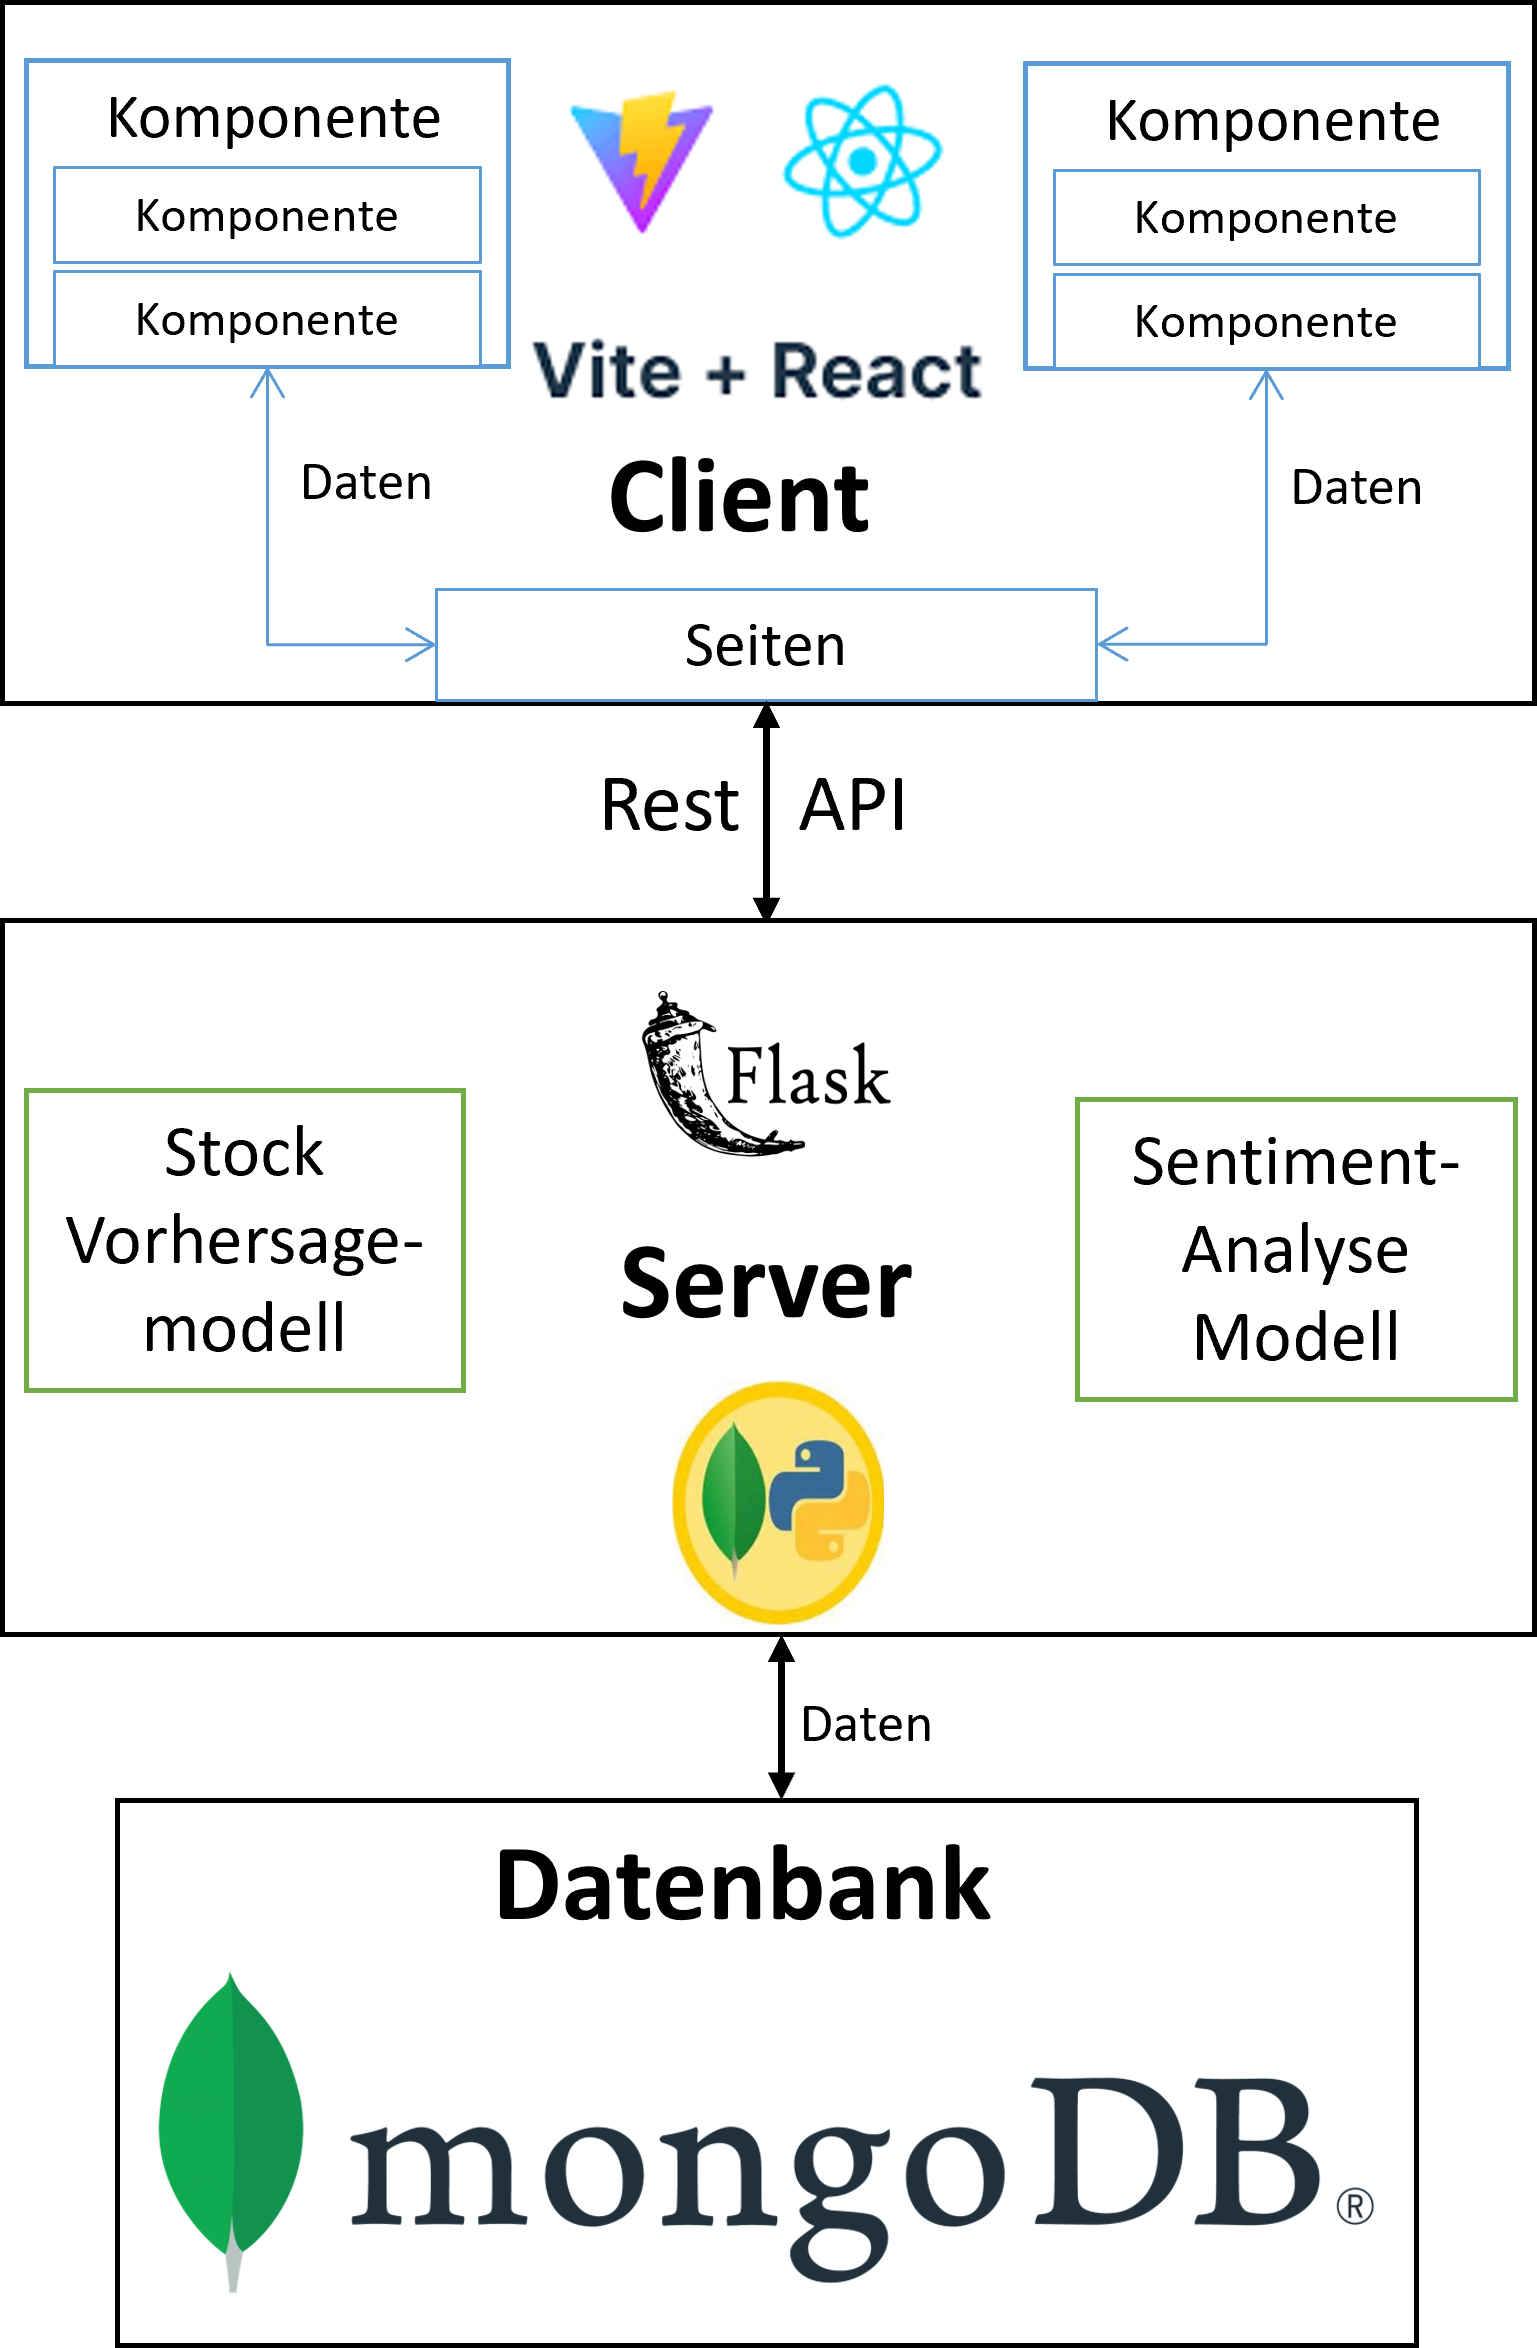
\includegraphics[width=0.9\linewidth]{TechStack.png}
    \caption{Technologie Stack}
\end{figure}


\subsection{Frontend}
Das Frontend der Webanwendung Musk Monitor bietet eine benutzerfreundliche und interaktive Oberfläche, die speziell für Trader und Analysten entwickelt wurde. Die Architektur basiert auf dem React-Framework, das eine effiziente Entwicklung und einfache Wartung ermöglicht, ergänzt durch moderne UI-Bibliotheken wie Material-UI für optimiertes Design und Benutzererfahrung.

Die zentrale Homepage führt die Nutzer übersichtlich durch die Anwendung. Von dort gelangen sie zu spezifischen Seiten, beispielsweise der Hauptansicht für Aktienprognosen. Diese Seite bietet einen interaktiven Aktienchart, bei dem Nutzer verschiedene Ansichten auswählen können, wie Eröffnungskurs, Tageshoch, Tagestief, Schlusskurs und Volumen. Nutzer können zudem den Zeitintervall flexibel einstellen, um die Daten ihren Analyseanforderungen anzupassen. Eine weitere Funktion ermöglicht es, zwischen dem realen Aktienchart und dem zusätzlich prognostizierten Chart zu wählen. Die Visualisierung erfolgt mithilfe von Recharts, wodurch historische und prognostizierte Aktienkurse dynamisch dargestellt werden. Tweets an Tagen mit besonders hohen Kursveränderungen werden hervorgehoben, um deren Einfluss besser zu veranschaulichen.

Zusätzlich integriert das Frontend eine Zeitachsen-Ansicht, die Elon Musks Tweets chronologisch anzeigt und um die jeweilige Sentimentbewertung ergänzt. Dies ermöglicht es den Nutzern, Korrelationen zwischen den Tweets und dem Verlauf der Aktienkurse intuitiv zu erkennen.

Die Kommunikation mit dem Backend erfolgt über eine RESTful API, um Daten wie historische Aktienkurse, Tweets und Sentimentanalysen abzurufen. Der Fokus des Musk Monitor-Frontends liegt auf einer intuitiven Bedienung, hoher Performance, modernem Design und dynamischen Visualisierungen, die alle relevanten Informationen kompakt und verständlich präsentieren.

\subsection{Backend} 
Das Backend der Anwendung wurde mit dem Flask-Framework implementiert, das eine einfache und effiziente Erstellung von Webanwendungen ermöglicht. Es verarbeitet Aktienkursdaten und führt Sentiment-Analysen auf Tweets durch. Flask arbeitet dabei in Kombination mit MongoDB, während die Sentiment-Analyse in einem separaten Modul ausgeführt wird. Das Flask-Anwendungsobjekt definiert die Routen für die Kommunikation mit dem Frontend.

Die MongoDB-Datenbank wird mithilfe des MongoClient aus der pymongo-Bibliothek angesprochen, um eine Verbindung zur externen Datenbank herzustellen, die die Aktieninformationen speichert. Zusätzlich zur Speicherung von Aktienkursen ermöglicht das Backend die Durchführung von Sentiment-Analysen für empfangene Tweets. Diese Analysen erfolgen über ein externes Modul, das die Sentiments bewertet und die Ergebnisse als JSON-Objekt zurückgibt. Bei ungültigen Anfragen wird ein Fehlerprotokoll erstellt, und der Nutzer erhält eine entsprechende Fehlermeldung.

Für Fehlerbehandlung und Überwachung verwendet die Anwendung das Python-Logging-Modul, das Fehler und Debug-Informationen protokolliert. Ein StreamHandler stellt sicher, dass die Logs in der Konsole sichtbar sind, was die Diagnose von Problemen und die Überwachung des Anwendungsstatus erleichtert. Die Log-Ebene ist auf DEBUG gesetzt, um detaillierte Informationen über alle durchgeführten Operationen zu speichern.

Zur Sicherstellung aktueller Aktienkursdaten nutzt das Backend das Python-Paket Flask-APScheduler. Täglich wird eine Funktion auf dem Webserver ausgeführt, die Tesla-Aktieninformationen von Alpha Vantage abruft und diese in der Datenbank speichert.




\subsection{Data Tier}
Aufgrund der heterogenen Daten und der guten Performance wird MongoDB als Persistenzschicht verwendet. MongoDB speichert Daten in Form von JSON-Objekten in Dokumenten. Tweets und Aktiendaten werden in separaten Dokumenten abgelegt: Ein JSON-Objekt für Tweets enthält den Zeitpunkt (Datum und Uhrzeit) sowie den Tweet-Text. Für Aktiendaten werden der Kurstag, Eröffnungs- und Schlusskurs, Tageshoch und -tief sowie das gehandelte Volumen gespeichert.

Um Tesla-Aktienkurse abzurufen, werden alle Daten aus der Datenbank als nach Datum sortierte Liste von JSON-Objekten zurückgegeben. Falls der Nutzer im Frontend einen bestimmten Zeitraum oder ein spezifisches Attribut der Aktiendaten (z.B. Tageshoch, -tief) auswählt, werden die Daten bereits beim Datenbank-Query entsprechend gefiltert. Die gleiche zeitbasierte Filterung ist auch für Tweets möglich.

Die Datenbank läuft in einem Docker-Container, der zustandslos ist. Das bedeutet, dass alle während der Laufzeit gespeicherten Daten beim Neustart des Containers verloren gehen würden. Dieses Problem wird durch ein Docker-Volume gelöst, das an den MongoDB-Container gemountet wird. Dadurch werden die Daten im Docker-Volume gespeichert, das unabhängig von der Laufzeit des Containers existiert und so die Persistenz der Datenbankinhalte sicherstellt.

Die Skalierbarkeit der Persistenzschicht wird mittels Sharding sichergestellt. Hierfür werden die Daten auf mehrere voneinander unabhängige Shards aufgeteilt. Dadurch enthält jede Shard nur einen Anteil an der Gesamtdatenmenge, wodurch die einzelnen Shards auf vielen leistungsschwächeren Rechnern ausgeführt werden können. Dieser Ansatz der Skalierung ist effizienter als eine MongoDB-Instanz auf einem leistungsstärkeren Rechner auszuführen, weil die Lese- und Schreiboperationen der einzelnen Shards parallel ausgeführt werden können. Die Kommunikation mit den Shards erfolgt über einen zentralen Router, der die Clientanfragen an die Shards mit den Daten weiterleitet und die Ergebnisse an den Client zurückgibt. Die Konfiguration des Routers und der Shards erfolgt über einen Config Server. Die einzelnen Shards bestehen aus einer primären und zwei sekundären MongoDB-Instanzen. Nur die primäre Instanz erhält Schreibbefehle, welche anschließend von den sekundären Datenbanken nachgemacht werden. Dadurch sind die Daten aller drei Instanzen immer untereinander synchron. Fällt die primäre Instanz aus, so bestimmen die verbleibenden sekundären Instanzen eine neue primäre Datenbank. Sowohl primäre, als auch sekundäre Instanzen können Lesebefehle ausführen, was die Leistungsfähigkeit bei unserer sehr leselastigen Anwendung verbessert.

\subsection{Deployment}
Das Deployment des Systems basiert auf einer GitLab-gestützten CI/CD-Pipeline, die alle wesentlichen Schritte von Build und Tests bis hin zur Bereitstellung automatisiert. Dies gewährleistet eine hohe Effizienz, Konsistenz und Skalierbarkeit in der Entwicklungs- und Bereitstellungsphase.

Die gesamte CI/CD Pipeline ist in GitLab implementiert und verwendet GitLab Runner. Die Pipeline besteht aus drei Hauptstages Build-Stage, Test-Stage und Deploy-Stage.
In der Build-Stage werden die Quellcodes mittels Docker in einer isolierten Umgebung gebaut. Hierbei wird eine reproduzierbare Umgebung sichergestellt, sodass der Build-Prozess unabhängig von der lokalen Entwicklungsumgebung der Entwickler ist.
Anschließend werden automatisierte Tests in einer Docker-Umgebung ausgeführt. Diese Tests decken sowohl Unit-Tests als auch Integrationstests ab und stellen sicher, dass der erstellte Build den Qualitätsanforderungen entspricht.
Nach erfolgreichem Abschluss der Tests, werden die Build-Artefakte in der Deploy-Stage auf den Zielserver übertragen. Der Zielserver basiert auf Ubuntu 22.04 und verwendet einen ARM-Prozessor.

\textbf{Deployment-Prozess:}
Das Deployment der Anwendung erfolgt in mehreren Schritten. Zunächst werden die getesteten Artefakte mithilfe des sicheren Übertragungsprotokolls SCP auf den Zielserver kopiert. Dadurch wird sichergestellt, dass die Dateien zuverlässig und geschützt übertragen werden.

Anschließend wird auf dem Zielserver Docker Compose verwendet, um die Anwendung zu starten. Docker Compose orchestriert dabei die verschiedenen benötigten Container und stellt sicher, dass alle Dienste korrekt miteinander interagieren. Dies erleichtert die Verwaltung von abhängigen Diensten sowie deren Konfigurationen und ermöglicht ein reibungsloses Deployment der gesamten Anwendung.

\textbf{Vorteile der Architektur:}
Die gewählte Architektur zeichnet sich durch ihre Portabilität aus. Dank Docker und Docker Compose ist die Lösung unabhängig von der zugrunde liegenden Infrastruktur und kann problemlos auf unterschiedliche Plattformen übertragen werden. Ein weiterer Vorteil ist die Automatisierung des gesamten Prozesses. Durch die GitLab-Pipeline wird der Ablauf von Build, Test und Deployment vollständig automatisiert, was den manuellen Aufwand erheblich reduziert und die Zuverlässigkeit erhöht.

Darüber hinaus sorgt die Nutzung von Containern für eine saubere Trennung der einzelnen Dienste. Dies erleichtert die Wartbarkeit der Anwendung und beschleunigt die Fehlersuche, da die isolierten Dienste einfacher zu analysieren und zu warten sind.
Nach dem erfolgreichen Deployment wird die Webseite durch Nginx als Reverse Proxy bereitgestellt und ist auf dem Ubuntu-Server erreichbar.

\section{Herausforderung}
Der Umgang mit Twitter-Daten stellte sich als unerwartet schwierig heraus. Nach der Einstellung der kostenlosen Twitter-API mussten alternative Methoden wie klassisches Web-Scraping oder der Zugriff auf andere APIs in Betracht gezogen werden. Allerdings erwiesen sich diese Ansätze als unzuverlässig oder wurden durch Sicherheitsmechanismen blockiert. Alternativen wie die Nitter-API funktionierten nur unregelmäßig, sodass für die Verarbeitung historischer Daten auf öffentliche Datensätze zurückgegriffen wurde.

Ein weiteres Problem zeigte sich bei der Aktien-API, die während der Entwicklung teilweise fehlerhafte historische Kursdaten lieferte. Um die Prognosegenauigkeit sicherzustellen, mussten korrekte historische Daten manuell aus NASDAQ-Exports bezogen und mit aktuellen Daten kombiniert werden.

Auch technologische Anpassungen waren notwendig. Die ursprüngliche Entscheidung, TensorFlow zu verwenden, führte zu Problemen auf macOS-Systemen mit M1-Chip. Dies machte eine vollständige Umstellung auf PyTorch erforderlich, um die Kompatibilität und Stabilität sicherzustellen.

Zusätzlich stellte die Teamgröße eine Herausforderung dar. Mit vielen Teammitgliedern war die Aufgabenzuweisung und Synchronisation komplex, was die Notwendigkeit klar definierter Rollen und effizienter Kommunikationsprozesse verdeutlichte.

Trotz dieser Herausforderungen konnte ein funktionsfähiges System entwickelt werden, das den geplanten Anwendungsfall erfolgreich abdeckt. Durch gezielte Lösungsansätze konnten die größten Hürden überwunden werden. Für zukünftige Projekte empfiehlt es sich, die Datenquellen und technischen Abhängigkeiten frühzeitig zu prüfen. Zudem sollten Mechanismen zur Skalierung von Teams sowie zur Sicherstellung der Datenqualität und -validierung von Beginn an etabliert werden.


\section{Ausblick}
In der aktuellen Implementierung basiert das Modell zur Aktienkursvorhersage ausschließlich auf historischen Kursdaten. Eine vielversprechende Erweiterung wäre die Integration zusätzlicher Datenquellen wie Tweets mit entsprechenden Sentimentanalysen, die zeitlich mit den Aktienkursen korrelieren. Durch die Einbeziehung von Stimmungen aus sozialen Medien könnte das Modell potenziell präzisere Vorhersagen treffen.

Aufgrund zeitlicher Einschränkungen im Projektverlauf konnte diese Idee bisher nicht vollständig umgesetzt werden, da die Synchronisation und korrekte Gewichtung der Sentiment-Daten eine komplexe Herausforderung darstellt. Die Integration von Sentiment-Daten stellt daher eine vielversprechende Richtung für zukünftige Verbesserungen dar, um das Modell weiter zu optimieren.

Des Weiteren werden akutelleim Frontend nur die neuesten 100 Tweets aus der Datenbank angezeigt. Eine Verbesserung könnte darin bestehen, die Tweets schrittweise nachzuladen. Anstatt alle 100 Tweets auf einmal anzuzeigen, könnten zunächst die letzten 30 Tweets geladen werden. Wenn der Nutzer weiter nach unten scrollt, können weitere 30 Tweets aus der Datenbank abgefragt und dynamisch angezeigt werden. Dieses sogenannte Lazy Loading würde die Performance der Anwendung verbessern und gleichzeitig ein flüssiges Nutzungserlebnis gewährleisten.

%%% Previous TechReps
%% INSTRUCTION: Remove the irrelevant ones and cite
%% the ones that are actually related on technological
%% level or that address the same domain.
%% (At the end, none of the \nocite is allowed,
%% just regular \cite commands within the mainmatter!)
%% This listing is just as a stimulus and reference:
%\cite{ModA-TR-2024SS-BCN-TeamRot-StockSentinel}
%\cite{ModA-TR-2023SS-BCN-TeamCyan-Stockbird}
%\cite{ModA-TR-2022SS-BDCC-TeamWeiss-TwitterDash}
%\cite{ModA-TR-2022SS-BDCC-TeamRot-Reddiment}

% ======== References =========
\sloppy
\printbibliography[notcategory=selfref]

\end{document}
